%!TEX root = FreeRtos ARM uController.tex
\subsection{Low Power Modes auf Stm32F4}
\label{sec:Low Power Modes}
Echtzeitbetriebssysteme kommen immer häufiger in akkubetriebenen embedded Systemen zum Einsatz. Solche Systeme verlangen eine effiziente Nutzung der Energieressourcen um einen möglichst langen Betrieb zu ge\-währ\-leis\-ten. Bezogen auf den $\mu$\-Pro\-zesso\-r gibt es im Prinzip zwei Wege Energie einzusparen:
\begin{itemize}
	\item Heruntertakten des $\mu$\-Pro\-zesso\-rs.
	\item Das System schlafenlegen, wenn keine weiteren Aufgaben anstehen.
\end{itemize}
Das Heruntertakten des $\mu$\-Pro\-zesso\-rs ist unabhängig vom Einsatz eines RTOS, daher werden wir hier nur den zweiten Punkt genauer betrachten, das Schlafenlegen des $\mu$\-Pro\-zesso\-rs. 
\begin{figure}[htb!]
	\centering
		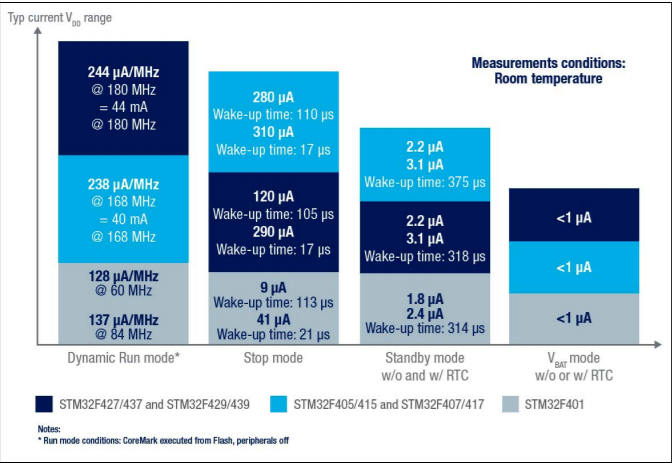
\includegraphics[width=0.4\textwidth]{Pictures/STM32F4/powerConsumption.png}
	\caption{Der STM32F4 bietet diverse LowPower Modes. Die Modes haben starke Auswirkung auf die Funktionalität des uControllers während der Schlafphase. Beispielsweise kann um Stop Mode keine UART Schnittstelle benutzt werden. Abhängig von der benötigten Peripherie, wählt der Entwickler einen dieser Modes. Die genutzte Taktfrequenz hat ebenfalls Einfluss auf die Stromaufnahme. Eine Anpassung der Takfrequenz zur Laufzeit ist ebenfalls möglich.}
	\quelle{STM32F4 - Power Modes}
	\label{fig:powerconsum}
\end{figure}
Abbildung \ref{fig:powerconsum} zeigt wie sich die Stromaufnahme beim STM32F4 von 40mA im Normalbetrieb(@168 MHz) auf 2,2$\mu$A im Tiefschlafmodus reduzieren lässt. 
In einfachen Anwendungen ist der Zustand in dem ein Gerät schlafen gehen kann relativ leicht zu ermitteln. In komplexen Systemen, die auf einem Echtzeitbetriebssystem wie FreeRTOS aufsetzen und mehrere Task mög\-li\-cherweise auf unterschiedliche Ressourcen warten, wird es schon schwierig. In diesem Abschnitt wird gezeigt welche Funktionen FreeRTOS zur Ver\-fü\-gung stellt, um einen energieeffizienten Betrieb zu ge\-währ\-leis\-ten. Eine Mög\-lich\-keit ist die Idle - Hook Funktion. Wie bereits in Abschnitt \ref{Scheduling} beschrieben, wird die IDLE Task von FreeRTOS aktiviert, sobald sich alle User-Tasks im Blocked Zustand befinden. Durch konfigurieren des Präprozessor-Defines        
\begin{lstlisting}[label=lst:defineIdleHook, numbers = none]
#define configUSE_IDLE_HOOK  1; 
\end{lstlisting}
\begin{lstlisting}[caption={Aufruf der IdleTask Hook Funktion durch die FreeRTOS Idle Task. Aus Task.c},captionpos=b, label=lst:xIdleTaskHook, float=htb!]
static portTASK_FUNCTION( prvIdleTask, pvParameters )
{
	/* Stop warnings. */
	( void ) pvParameters;

	/** THIS IS THE RTOS IDLE TASK - WHICH IS CREATED AUTOMATICALLY WHEN THE
	SCHEDULER IS STARTED. **/

	for( ;; )	{
//skipped some code
if ( configUSE_IDLE_HOOK == 1 )
{
	extern void vApplicationIdleHook( void );
	vApplicationIdleHook();
}
//guess what.. skipped more code
}     
\end{lstlisting}
kann die Idle-Hook Funktion aktiviert werden. Diese wird immer aufgerufen, sobald die Idle Task in den Zustand Running wechselt. Die Funktionalität der Idle-Hook Funktion kann frei vom Entwickler implementiert werden. 
\begin{lstlisting}[caption={Pseudocode für eine Idle Hook Funktion},captionpos=b, label=lst:xIdleHookExamp, float=hbt!]
extern "C" void vApplicationIdleHook( void ){
	/* Systick Interrupt deaktivieren */
	SysTick->CTRL &= ~SysTick_CTRL_TICKINT_Msk;
	//RTC konfigurieren
	setRTCWakeupTime();
	//externen Interrupt durch RTC aktivieren
	enableRTCInterrupt();
	//deaktiviere alle anderen Interrupt Quellen
	deactivateExternalDevices();
	setAllGPIOsToAnalog(); 
	disableGPIOClocks();
	//MCU stoppen und schlafen ZzZZz
	HAL_PWR_EnterSTOPMode(PWR_LOWPOWERREGULATOR_ON, PWR_STOPENTRY_WFI); 
	//Aufgewacht...the show must go on
	//aktiviere Systick
	SysTick->CTRL |= SysTick_CTRL_TICKINT_Msk;
	//reaktiviere GPIO Clocks
	enableGPIOClocks();
	//reaktiviere Externe Interrupt Quellen
	enableExternalInterrupts();	
}
\end{lstlisting}
Listing \ref{lst:xIdleHookExamp} zeigt Pseudocode zu einer beispielhaften Implementierung der Idle Hook Funktion. Bevor das System schlafen gelegt werden kann müssen alle GPIOS und IRQs konfiguriert werden, so dass das System nicht unnötiger weise aufwacht. Des Weiteren werden alle nicht benötigten GPIOS auf Analog gestellt um Energie zu sparen. Als einzige Interrupt-Quelle wird hier eine externe RTC konfiguriert. Mit dem Aufruf von HAL\_PWR\_EnterSTOPMode() wird der $\mu$\-Pro\-zesso\-r in den Schlafmodus versetzt. Die Funktion wird erst wieder verlassen sobald der externe Interrupt der RTC ausgelöst wurde. Danach werden alle GPIOs rekonfiguriert. Ein weiterer Schritt der noch unternommen werden muss ist das Informieren einer User-Task z.B. mittels Notify oder Message, so dass das System nicht beim nächsten Tick Interrupt wieder die Idle Task aktiviert. Nachteil dieser Variante ist, dass die Nutzung von Software Timer nicht mehr möglich ist. Der FreeRTOS Kernel würde die Idle Hook Funktion auch aufrufen und sich schlafen legen, wenn noch Software Timer aktiv sind. Die Nutzung von absoluten Zeiten ist ebenfalls nicht mehr möglich, da nach der Deaktivierung des Tick Interrupts der Tickcount nicht mehr korrekt ist. Abhilfe schafft hier eine weitere Funktionalität die FreeRTOS zur Verfügung stell, den sogenannten Tickless Idle Mode. Tickless idle kann durch das folgende Define in der FreeRTOSconfig.h aktiviert werden.  
\begin{lstlisting}[label=lst:defineTicklessIdle, numbers = none]
#define configUSE_TICKLESS_IDLE  1; 
\end{lstlisting}
Im Gegensatz zur gewöhnlichen Idle Hook Funktion be\-rück\-sich\-tigt der Tickless Idle Mode alle ausstehenden Timerfunktionen, dazu gehören alle Software Timer aber auch Tasks die nur für eine gewisse Zeit blockiert sind z.B. durch die Funktion xTaskWaitUntil(). Des Weiteren muss der Tickinterrupt nicht wie in Listing \ref{lst:xIdleHookExamp} explizit abgeschaltet werden, dies wird hier automatisch durch den Kernel gehandelt. Der Tickless Idle Mode bietet durch die Funktion vTaskStepTick() auch die Möglichkeit den TickCount nach dem Aufwachen anzupassen. Die verpassten TickCounts können beispielsweise durch einen externen Timer oder RTC bestimmt werden. So ist es auch möglich Software Timer für absolute Zeiten zu nutzen. Details und Beispiel Implementierungen hierzu findet man unter \cite{FreeRtosAdvanced}.  

